\documentclass[11pt]{article}
\usepackage{amsmath,amssymb,amsthm}
\usepackage[pdftex]{graphicx}
\usepackage{fancyhdr}
\pagestyle{fancy}

\setlength{\headheight}{0.75in}
\setlength{\oddsidemargin}{0in}
\setlength{\evensidemargin}{0in}
\setlength{\voffset}{-1.0in}
\setlength{\headsep}{10pt}
\setlength{\textwidth}{6.5in}
\setlength{\headwidth}{6.5in}
\setlength{\textheight}{8.5in}

\lhead{}
\chead{Guided Capstone Project Report}
\rhead{Jim Tao}
\lfoot{}
\cfoot{}
\rfoot{\thepage}
\renewcommand{\headrulewidth}{0.5pt}
\renewcommand{\footrulewidth}{0.3pt}
\setlength{\textwidth}{6.5in}

\begin{document}
\begin{flushleft}
{\em What opportunities exist for Big Mountain Resort to increase profits by
cutting costs without undermining ticket price or making investments that
support a higher ticket price?}
\end{flushleft}

Data wrangling shows us that the target feature to predict is ``AdultWeekend''
ticket prices, and exploratory data analysis comparing with statewide features
shows that it makes sense to treat all states equally and work towards
building a pricing model that considers all states together. Applying and
comparing two machine learning techniques, we find that random forest
regression is more accurate than linear regression and has better consistency
between cross-validation results and performance on the test set.

We are able to model the four following scenarios corresponding to business
strategies shortlisted by the business:
\begin{enumerate}
\item permanently closing down up to 10 of the least used runs
\item increasing the vertical drop by adding a run to a point 150 ft lower down
but requiring the installation of an additional chair lift to bring skiers
back up, without additional snow making coverage
\item same as number 2 but adding 2 acres of snow making cover
\item increase the longest run by 0.2 miles to boast 3.5 miles length,
requiring an additional snow making coverage of 4 acres
\end{enumerate}

Big Mountain currently charges \$81 for an AdultWeekend ticket. According to my modeling, a ticket price of \$95.87 could be supported in the marketplace
by Big Mountain's facilities. The additional operating cost of a new chair lift
is \$1,540,000, but per ticket it is less than \$1 because installing it,
opening a new run, and increasing the vertical drop by 150 feet supports
a price increase of \$1.99 that would account for an increase in revenue
of \$3,474,638. Therefore scenario 2 should definitely be taken into further
consideration for future improvements.
\begin{center}
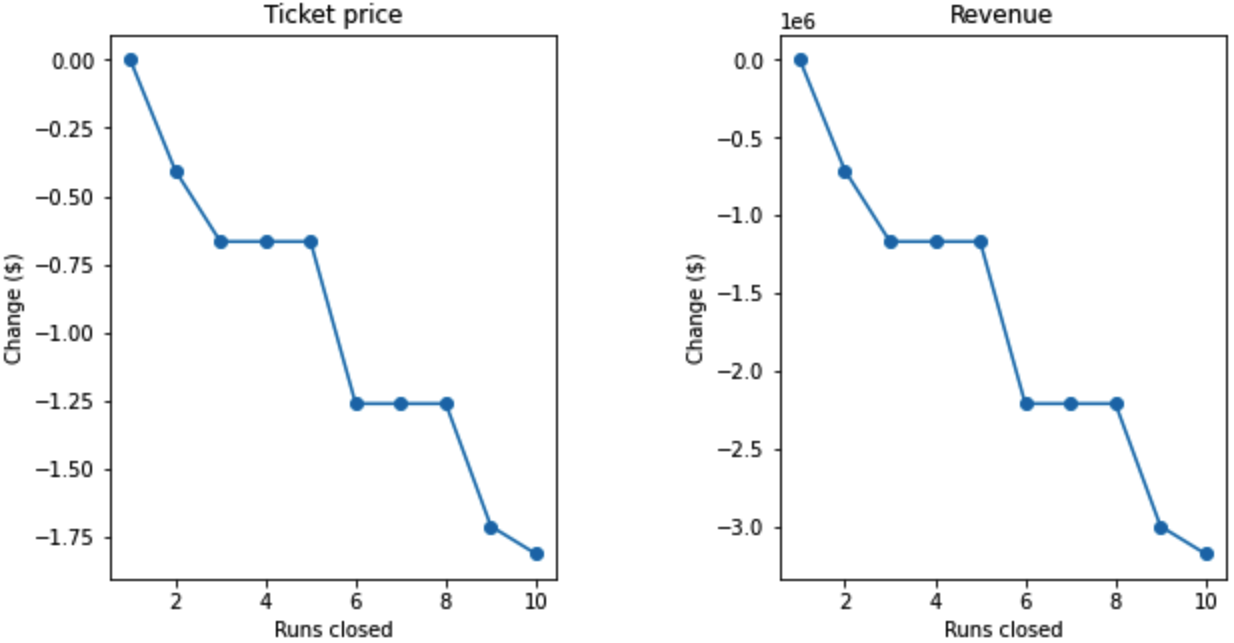
\includegraphics[scale=.25]{effectofclosingrunsonmarketpriceandrevenue}
\end{center}
Also, it may be possible to cut costs by closing runs without losing too
much revenue. From the data, it is not obvious what are the operational
costs associated with features other than chair lifts, but if the reduction
in operating costs from closing runs more than compensates for reduced
revenue from a lower market price for the tickets, it may also be worth
it to take into consideration scenario 1.
\end{document}
